\chapter{问题定义与语义关联度计算框架}
\label{chap:chap02}
本章着重介绍了语义关联度计算以及知识关联网络构建过程中的概念,然后综合考虑词语层与实体层的语义信息,详细阐述了知识关联网络驱动下的语义关联度计算框架。

\section{问题定义}
本节结合相关例子给出语义关联度和语义相似度的区别,然后针对知识关联网络中的相关概念给出其定义。表格~\ref{symbols}给出了本文所使用的符号以及其对应的含义。
\begin{table}[!ht]
    \center
    \smallcaption{本文所用符号及其对应含义}
    \vspace{5pt}
    \begin{tabular}{|p{2.5cm}|p{9cm}|}
    \hline
    \bf{符号} & \bf{含义} \\ \hline
    $KAN$ & 知识关联网络 Knowledge Association Network \\ \hline
    $G = (W, E, R)$ & 词集合$W$, 知识库实体集合$E$ 以及边集合$R$构成的图\\ \hline
    $G_{\{attr, t\}}$ & 图属性空间 $G_{attr}$和图拓扑空间$G_t$ \\ \hline
    $R_{\{w,we,e\}}$ & 知识关联网络中的三种边类型 \\ \hline
    $f_{\{w,we,e\}}$ & 针对知识关联网络中三种边的三种关联度度量方法 \\ \hline
    $W_{\{cnt,tf\_idf\}}$ &图$G_t$中两种衡量节点之间转移概率的方式\\ \hline
    $e(w)$ & 与词$w$相关的实体集合 \\ \hline
    $\mathbb{R_a}$ & 图属性空间在向量空间的表示 \\ \hline
    $\mathbb{R_t}$ & 图拓扑结构空间在向量空间的表示 \\ \hline
    \end{tabular}
    \label{symbols}
\end{table}


\subsection{语义关联度}

语义度量主要包含语义关联度和语义相似度,其中语义相似度主要考虑词语之间的种属关系~\cite{geoinformatica/BallatoreBW14},语义关联度则在相似度的基础上还要考虑更多的语义信息,比如反义、部分整体以及很多无法准确归类的潜在语义信息。这里通过一个简单例子描述两者的区别。如图\ref{chap2-1}所示,对于给定的三个词,左边表示人为标注的关联度数值,右边表示这三个词语在词法库中的层次关系。Bus(公共汽车)和 Train(火车)同时作为机动型交通工具拥有最高的关联度数值,而Bicycle(自行车)和Bus,人们经常考虑选择这两种交通方式短途出行,所以比Bicycle和Train之间的关联程度高。而仅仅考虑词语之间的种属关系时,即在图\ref{chap2-1}右侧的种属词法关系中,Train与Bicycle之间的距离要小于Bicycle与Bus之间的距离,也就是Train和Bicycle之间具有更高的语义相似度。综上所述,我们给出两者的定义:

\begin{figure}[!htb]
    \centerline{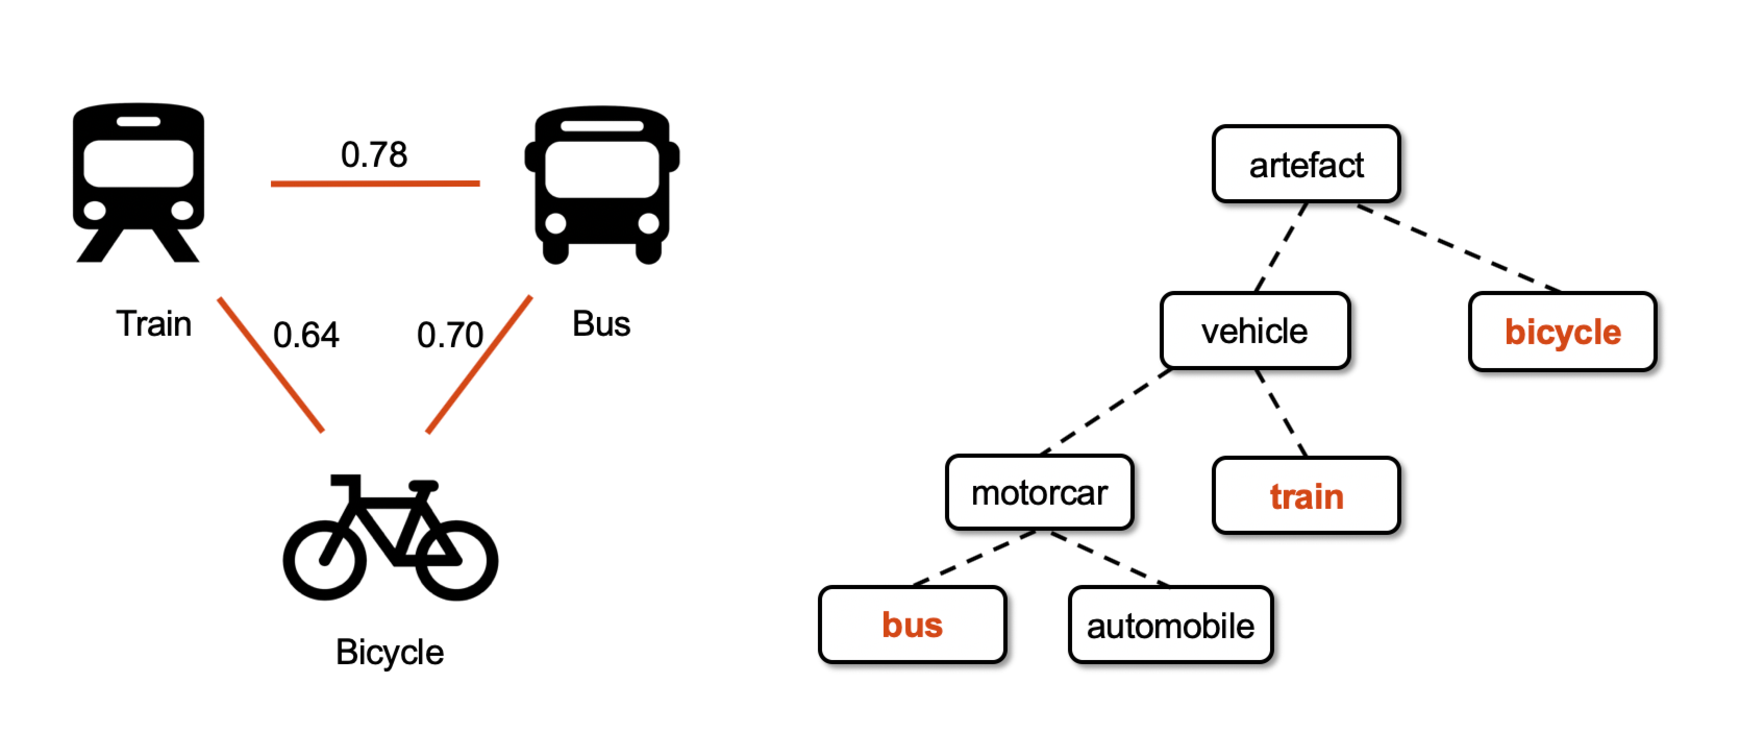
\includegraphics[width=0.9\textwidth]{chap2-1.pdf}}
    \smallcaption{语义关联度与语义相似度区别}
    \label{chap2-1}
\end{figure}

\begin{definition}
    \label{sr}
    {\bf 语义关联度(Semantic Relatedness)}
    对于给定的一对词语$w_1$和$w_2$,他们之间的语义关联度指通过比较$w_1$和$w_2$的语义表征之后,给出的其背后包含的意义或其语义内容之间的相关程度。这种相关程度的度量不仅仅要考虑其含义之间的种属关系,也要考虑其含义之间的其他复杂语义联系,比如部分整体关系、反义关系甚至一些无法准确描述的潜在语义关系。
\end{definition}

\begin{definition}
    \label{ss}
    {\bf 语义相似度(Semantic Similarity)}
    对于给定的一对词语$w_1$和$w_2$,他们之间的语义相似度指通过比较$w_1$和$w_2$在词法库或其隐藏在其他知识库中实体之间的种属关系之后给出的数值评分。相比于语义关联度,语义相似度考虑的词语间关系更加明确。
\end{definition}

\subsection{知识关联网络}
本文利用词语背后隐含的语义内容以及词语之间的共现关系来构建知识关联网络,并用来计算语义关联度。有了清晰的词语间语义关联度的概念之后,本节接下来阐述知识关联网络的相关概念。知识关联网络的构建依赖于知识库的选择,在第\ref{chap:chap01}章中给出的结构化知识库中,如本体库、知识图谱等,其中数据往往以RDF三元组的形式给出,其中三元组和RDF分别指:

\begin{definition}
    \label{rdf}
    {\bf 资源描述框架(Resource Description Framework,RDF)}
    是由万维网联盟(W3C)\footnote{https://www.w3.org/}提出的一组标记语言的技术规范,以便更为丰富地描述和表达网络资源的内容与结构,形式上表现为三元组。
\end{definition}

\begin{definition}
    \label{triple}
    {\bf 三元组(Triple)}
    是描述客观事物或抽象概念的一种方式,形式上表现为主语-谓语-宾语(Subject-Predicate-Object,SPO)。其中主语与宾语分别表示实体对象,而谓语表示连接主语与宾语的关系属性或类别。举个例子来说,\emph{\underline{Bus}(Subject) \underline{is a}(Predicate) \underline{vehicle}(Object)}或者\emph{\underline{Apple company}(Subject) \underline{produces}(Predicate) \underline{iPad}(Object)}。
\end{definition}

但是,对于一类对象以及这类对象的所属属性,RDF作为一种基础数据模型,表达能力有所不足,举个例子来说:\emph{“Yaoming is a basketball player”}和\emph{“Yaoming was born in Shanghai”},对于这样两条事实,RDF可以清晰的定义。但是对于定义\emph{“Yaoming is a person”},\emph{“Shanghai is a city”}以及\emph{person}和\emph{city}这两个对象各自的属性以及他们之间的联系时,不同的研究者会定义不同的属性和联系。为了规范化RDF数据的定义,RDFS(Resource Description Framework Schema)\footnote{https://www.w3.org/TR/rdf-schema/}和OWL(Web Ontology Language)\footnote{https://www.w3.org/OWL/}被提出建立起模式或者原语(Ontology)的概念来定义抽象化实体的属性以及他们之间的联系。

有了以上的这些基础之后,对于以RDF数据模式或其他形式存储的知识库,我们可以通过建立知识库实体与词语之间的联系来构建知识关联网络,这里给出其形式化定义:
\begin{definition}
    \label{kan}
    {\bf 知识关联网络(Knowledge Association Network,KAN)}
    知识关联网络有效地连接起词语与其背后包含的意义之间的联系,其本质上表现为一张图$G=(W, E, R)$,如图\ref{chap1-2}所示,其中$W$为词典中的词语集合,$E$是与$W$中所有词相关联的知识库实体所构成的集合,这样$W$和$E$组成了知识关联网络中的节点集合。而对于边集合$R$, 在KAN中分为三种:词语之间的关系$R_w$、实体之间的关系$R_e$以及词语与实体之间的关系$R_{we}$。
\end{definition}


\section{知识关联网络驱动的语义关联度计算框架}
\label{chap02-sr}
当明确语义关联度与知识关联网络的相关概念之后,本节从整体上介绍如何统筹知识关联网络中边的三种类型来计算最后的关联度值。

\begin{figure}[!ht]
    \centerline{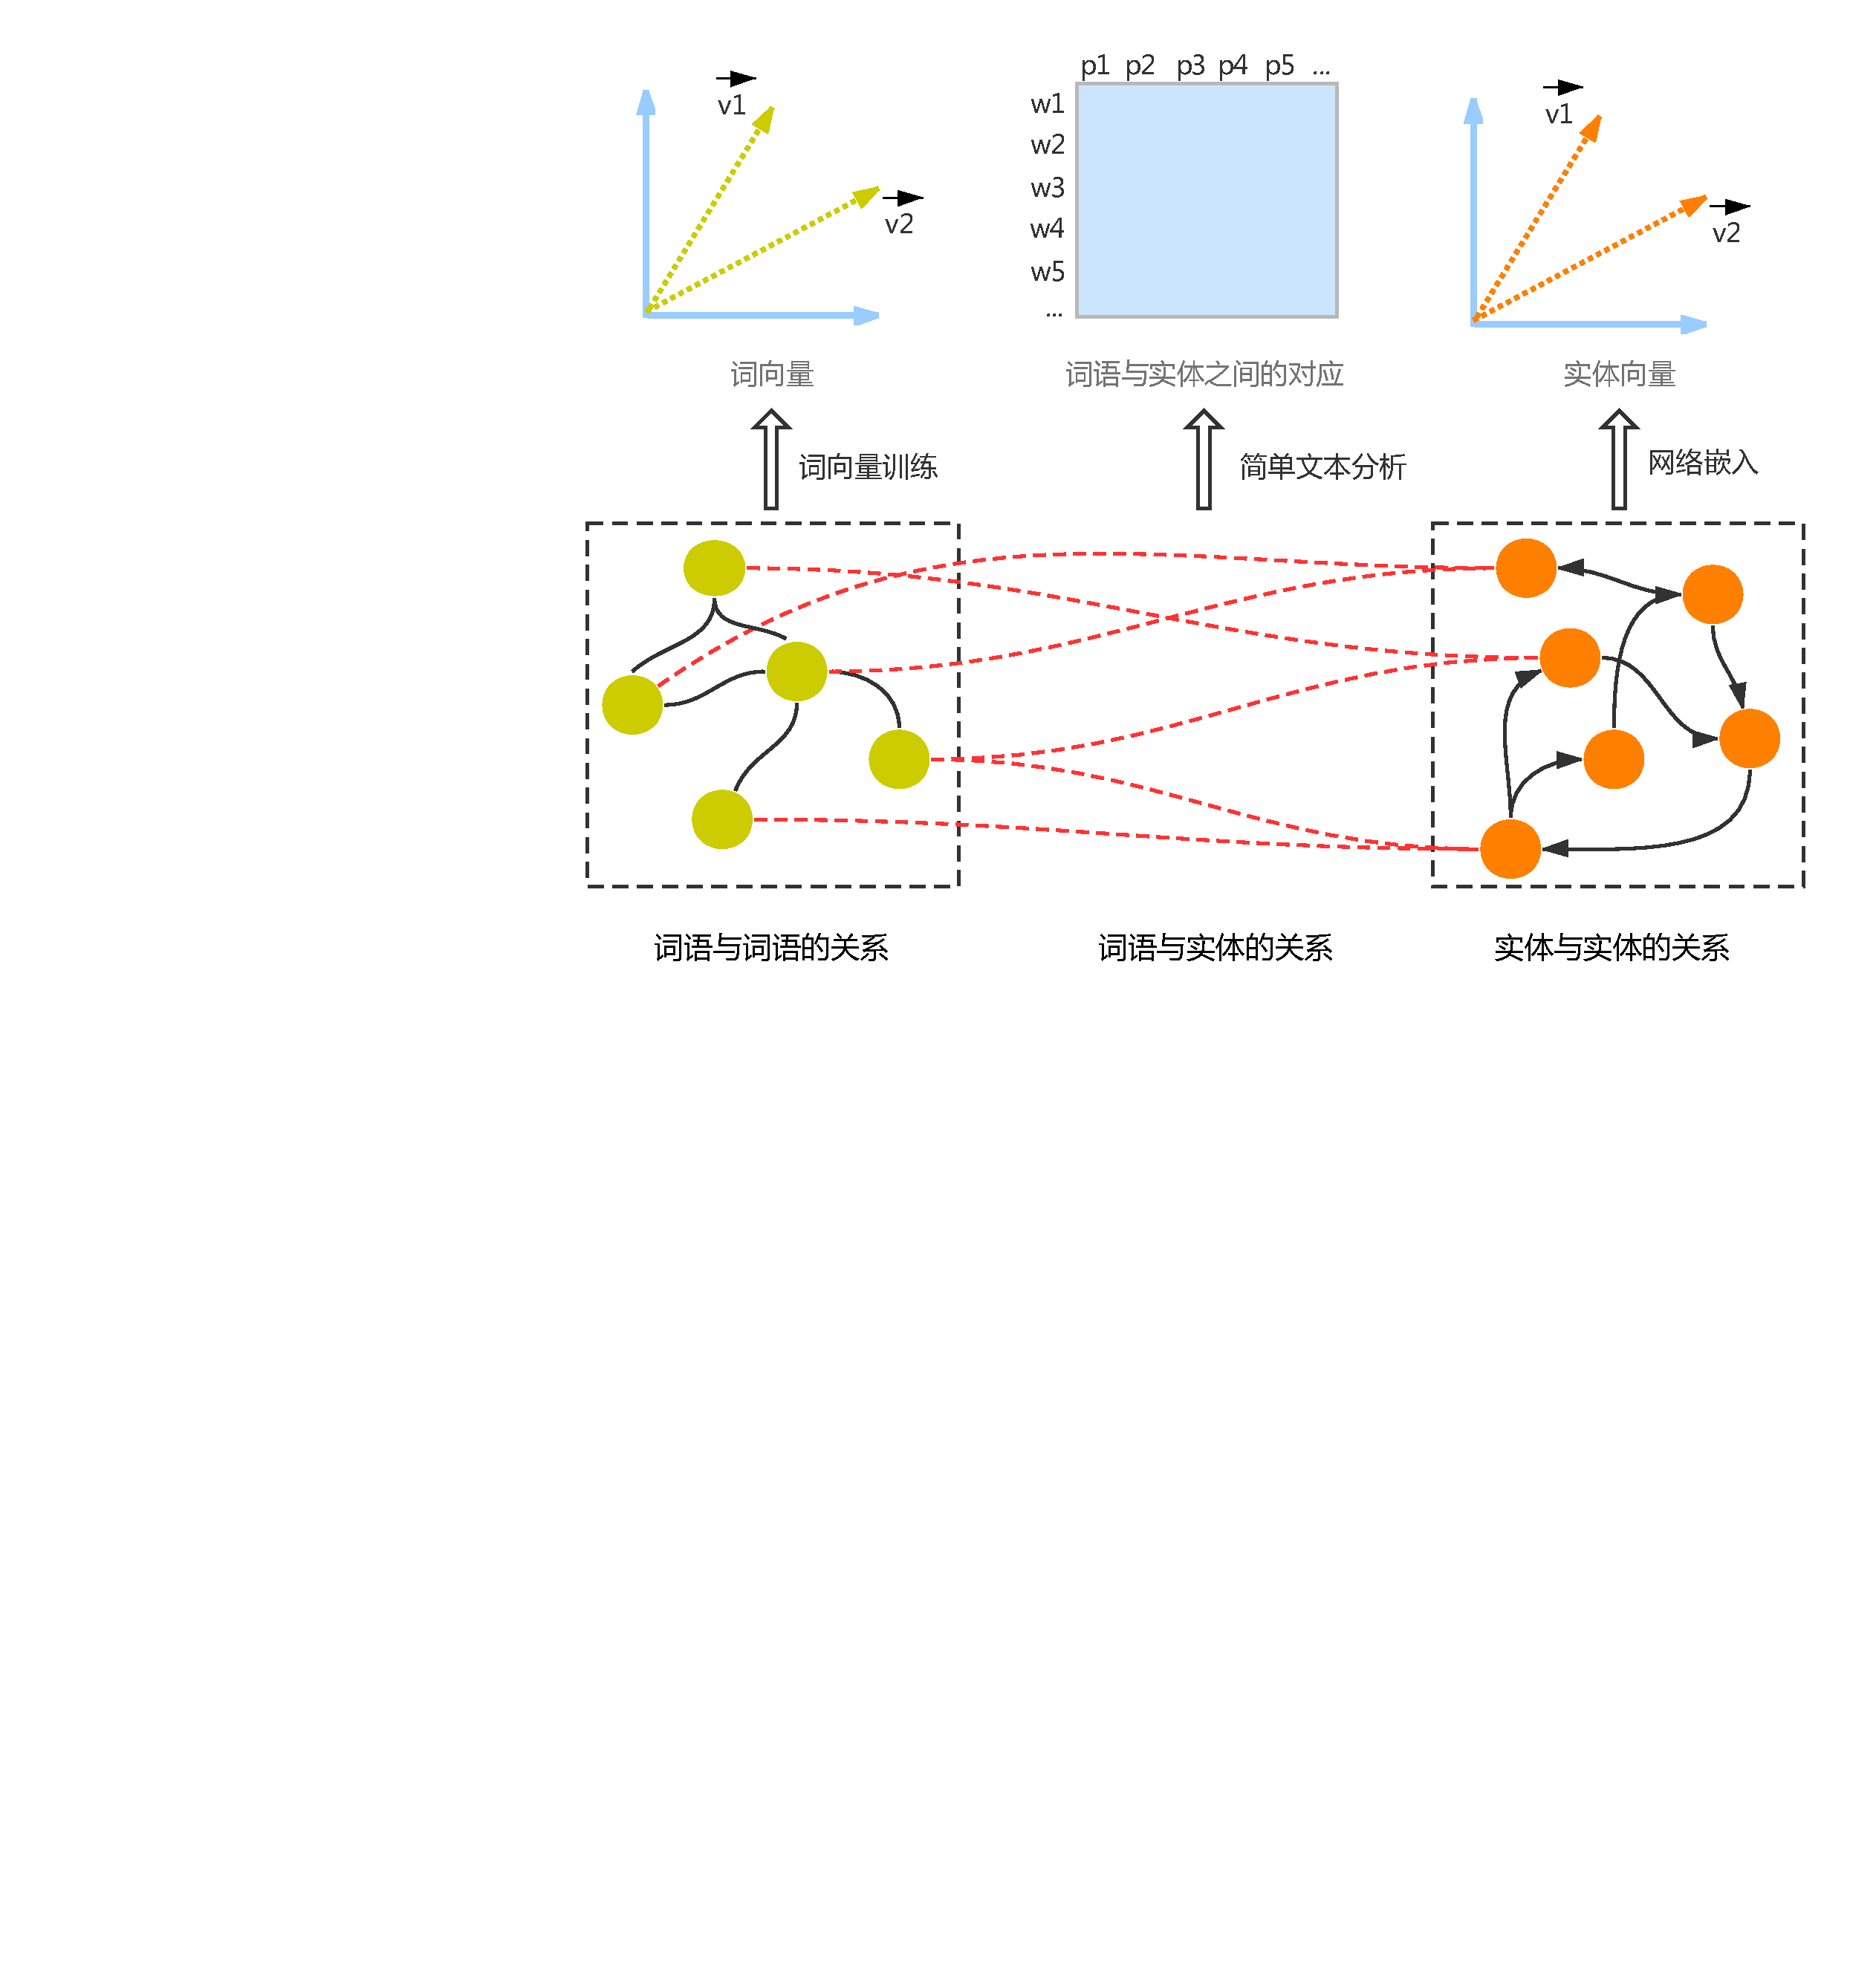
\includegraphics[width=0.8\textwidth]{chap2-2.pdf}}
    \smallcaption{知识关联网络三种边类型对应的处理方法}
    \label{chap2-2}
\end{figure}

如图\ref{chap2-2}所示,对于知识关联网络中的三种关系,我们可以通过不同的方法得到他们之间的数值关联程度。1)词语与词语之间的关系反映了语料库中词语之间的共现关系。这部分我们主要通过词向量训练模型来得到对应的词向量表示,然后通过向量距离计算来得到词语层$w_i$和$w_j$之间的关联度,记为$f_w(w_i, w_j)$;2)词语与实体之间的关系主要起到连接词语层与知识库实体的作用,可以根据词语与实体之间的不同的相关程度得到不同的权重。这部分主要通过文本匹配等简单的处理来建立词语与实体之间的关系,而至于某条关系的权重,记录为$f_{we}(w, e)$,针对不同的知识库选择,关系权重的分配方法不同,本文将在接下来的两章做阐述。3)实体与实体之间的关系反映了词语与实体之间的联系,这部分主要通过不同的网络嵌入模型来学习实体的分布式向量表征,然后实体之间的相似度也可以被快速计算得到,记为$f_{e}(e_i, e_j)$。

当得到知识关联网络中三种关系连接的主体之间的关联度后,本文将最终词语间语义关联度分为两部分:词语层的语义关联度和实体层的语义关联度。对于词语层的语义关联度,本文直接采用词语与词语之间的向量距离作为最终结果,即:
\begin{equation}
F_w(w_i, w_j) = f_{w}(w_i, w_j)
\label{F_w}
\end{equation}

\noindent 对于实体层的语义关联度,本文通过组合词语与实体以及实体与实体之间的关系来计算,如图\ref{chap2-3}所示对于两个词语$i$和$j$,通过其相关实体而连接起两个单词的路径有多条,图中有12条。而对于两个词语$i$和$j$在一条由实体$m$和$n$连通的路径上的关联度,我们可以通过下面的方法得到:
\begin{equation}
    W_{path}(w_i, w_j, e_m, e_n) = f_{we}(w_i, e_m)f_e(e_m, e_n)f_{we}(w_j, e_n)
    \label{wpath}
\end{equation}

\noindent 由此,词语在实体层面的语义关联度可以按照如下公式计算:
\begin{equation}
    F_e(w_i, w_j) = \mathscr{F}_{e_m \in E_i,e_n \in E_j}W_{path}(w_i, w_j, e_m, e_n)
    \label{F_e}
\end{equation}

\begin{figure}[!ht]
    \centerline{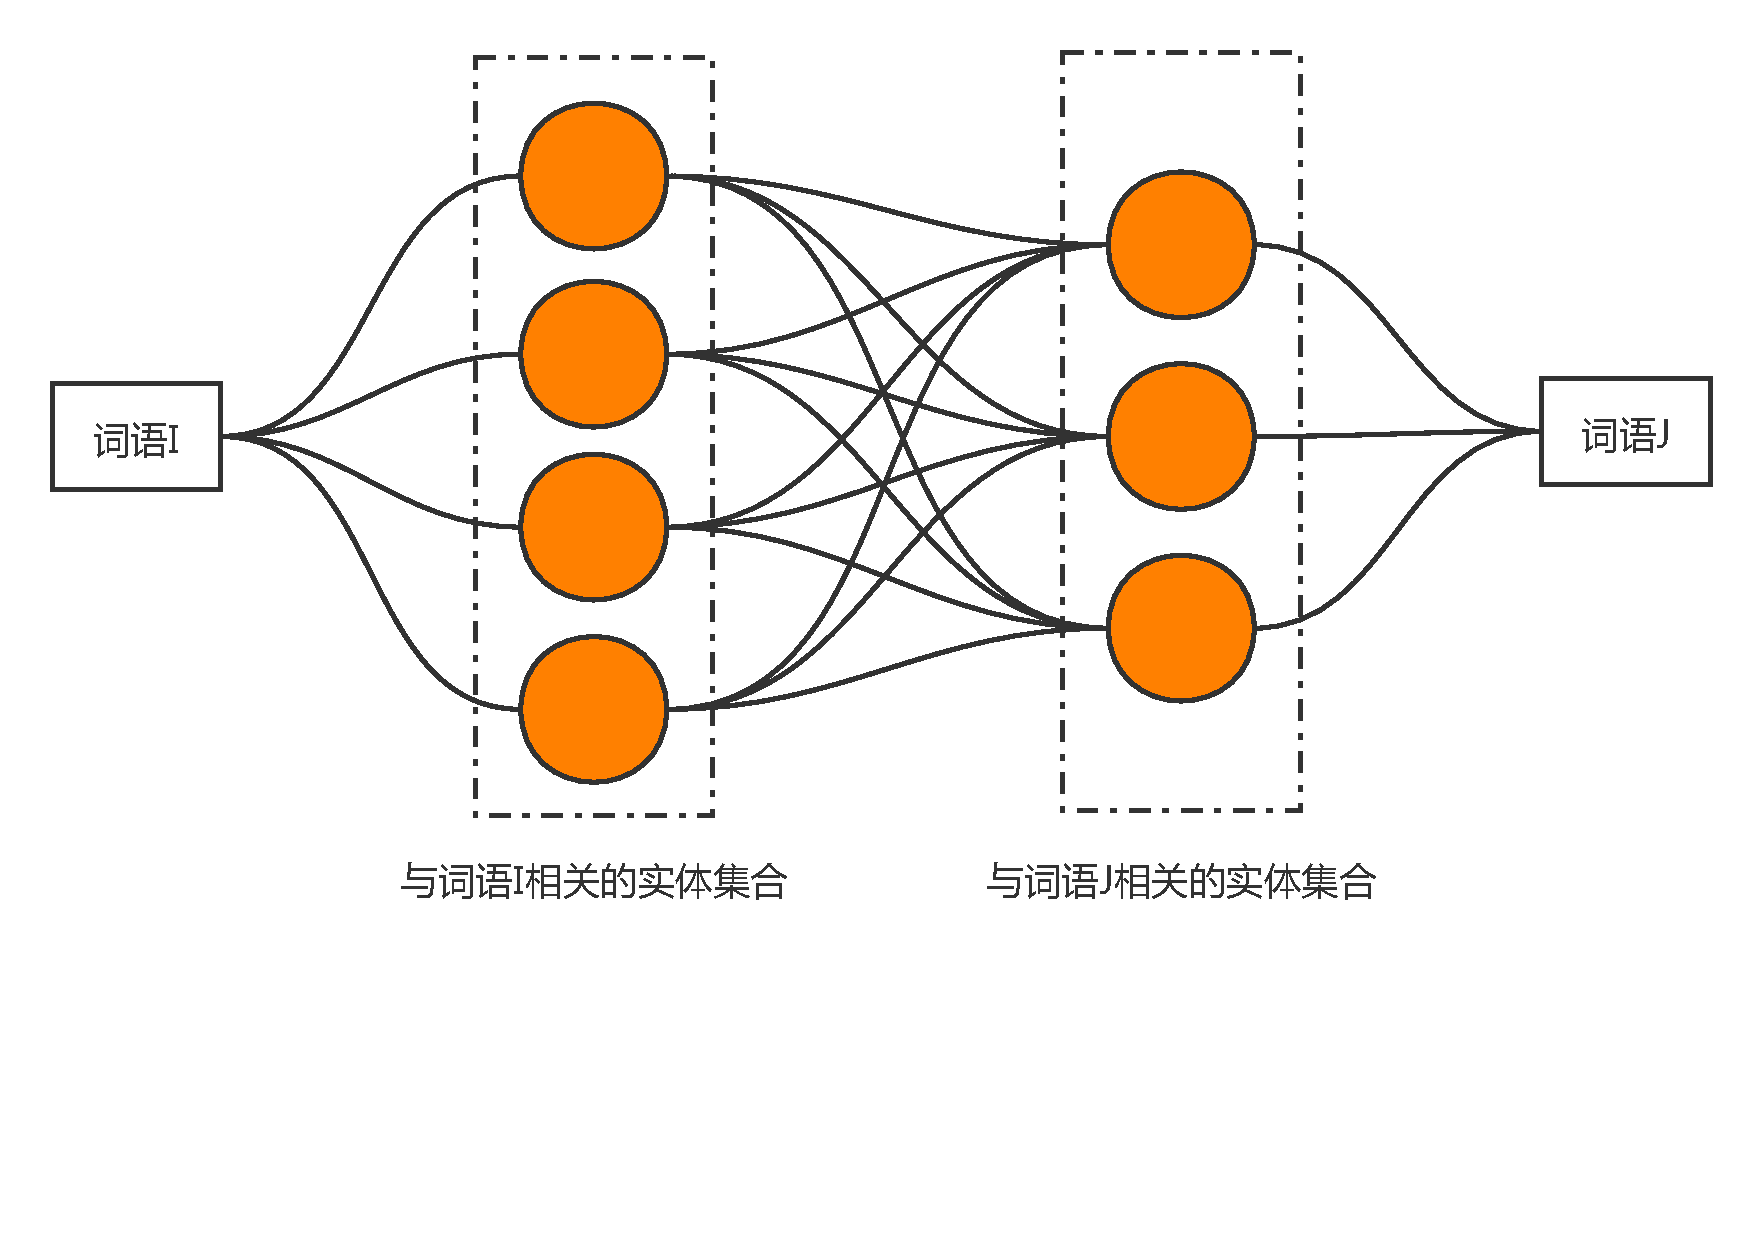
\includegraphics[width=0.8\textwidth]{chap2-3.pdf}}
    \smallcaption{实体层语义关联度度量示例}
    \label{chap2-3}
\end{figure}

\noindent 其中,$E_i$表示与词语$w_i$有连接的所有实体集合,$E_j$类似。而$\mathscr{F}$表示聚合策略,即针对词语之间由相关联实体所构成的多条路径所采用的聚合方法。聚合方法的采用视情况而定,经常采用的的是求平均值的方法,对应公式如下:
\begin{equation}
    F_{e;avg}(w_i, w_j) = \sum_{e_m \in E_i}^{ }\sum_{e_n \in E_j}^{ }W_{path}(w_i, w_j, e_m, e_n)
    \label{F_e_avg}
\end{equation}

\noindent 特殊的,当词语与实体层之间的边权重无法准确衡量时,本文还采用了取实体间关联度最大值的策略来衡量词语在实体层的语义信息:
\begin{equation}
    F_{e;max}(w_i, w_j) = \max_{e_m \in E_i,e_n \in E_j}f_e(e_m, e_n)
    \label{F_e_max}
\end{equation}

\noindent 最后可以得到最终的词语间语义关联度为:
\begin{equation}
    F(w_i, w_j) = \varphi F_w(w_i, w_j) + (1 - \varphi) F_e(w_i, w_j)
    \label{F}
\end{equation}

\noindent 其中$\varphi$取值空间为$[0,1]$,起到了平衡词语层语义关联度$F_w$和实体层语义关联度$F_e$的作用。最后我们给出整个过程的算法流程:

\begin{algorithm}
    \smallcaption{知识关联网络驱动的语义关联度计算流程}
    \label{alg:kan-sr}
    \SetKwInOut{Input}{输入}
    \SetKwInOut{Output}{输出}
    \SetKw{Return}{return}
    \Input{KAN, 词语$w_i$, $w_j$, 预训练词向量$v_w$, 实体向量$v_e$, 词语与实体间的关联值$f_{we}$, $\varphi$}
    \Output{语义关联度值$F{(w_i,w_j)}$}
    \BlankLine
    查询KAN得到$w_i$和$w_j$的关联实体集合$e(w_i), e(w_j)$ \;
    $F_w(w_i, w_j) \leftarrow f_w(w_i, w_j) \leftarrow cos(\vec v_{wi},\vec v_{wj})$ \;
    \For{$e_m \in e(w_i)$, $e_n \in e(w_j)$} {
        $f_e(e_m, e_n) \leftarrow cos(\vec v_{em},\vec v_{en})$ \;
        $W_{path}(w_i, w_j, e_m, e_n) \leftarrow f_{we}(w_i, e_m)f_e(e_m, e_n)f_{we}(w_j, e_n)$; \;
    }
    $F_e(w_i, w_j) \leftarrow \mathscr{F}_{e_m \in E_i,e_n \in E_j}W_{path}(w_i, w_j, e_m, e_n)$ \;
    $F(w_i, w_j) \leftarrow \varphi F_w(w_i, w_j) + (1 - \varphi) F_e(w_i, w_j)$ \;
    \Return $F(w_i, w_j)$
\end{algorithm}

\section{本章小结}
本章首先通过一个简单的例子阐述了语义关联度和语义相似度的区别并给出了定义,随后对知识库的主要数据存储模式RDF做了简要阐述。有了这些基础之后,本章还介绍了如何组合知识关联网络中的三种关系来计算最终的语义关联度,并给出了算法流程。
